%!TEX root = "../../DA_GUI.tex"
%	########################################################
% 				Allgemeiner Teil (Theorie)
%	########################################################


%	--------------------------------------------------------
% 	Aufbau der Benutzeroberfläche
%	--------------------------------------------------------


\chapter{Die Benutzeroberfläche der Entwicklungsumgebung}
\label{sec:gui-main}
Zu diesem Bereich zählen alle Elemente des Hauptfensters. Der Grundlegende Aufbau wurde bereits vor dem Projektstart entworfen und in unserem Praktikum im Sommer 2014 implementiert. Vom Herbst 2014 bis Ende Januar 2015 wurde der Aufbau und die Bedienung dieser Oberfläche erweitert und verbessert. Eine besondere Hilfestellung dabei waren die Versuche mit SchülerInnen der ersten und zweiten Klassen, die an unseren Versuchen teilgenommen haben.
%TODO reference versuche

%TODO list parts of GUI

%TODO refer to package "at.jku.ssw.cmm.gui.*"

%TODO describe how to launch C Compact (from class...)

%TODO add desc for GUIExecutable

\section{Basispanel des Hauptfensters}
\ref{sec:gui-main}
Die Entwicklungsumgebung selbst ist in zwei Hälften geteilt. Im Linken Teil befinden sich die Textfelder für den Quelltext und für die Ein- und Augabe des CMM-Programmes. Im rechten Teil befinden sich Registerkarten mit unterschiedlichen Aktionsfeldern.

Die beiden Teile sind durch einen Balken getrennt, der mit der Maus verschoben werden kann. Diese Funktionen wurden mit dem Swing-Element JSplitPane\footnote{http://docs.oracle.com/javase/7/docs/api/javax/swing/JSplitPane.html} implementiert.

\begin{figure}[htbp] 
  \centering
     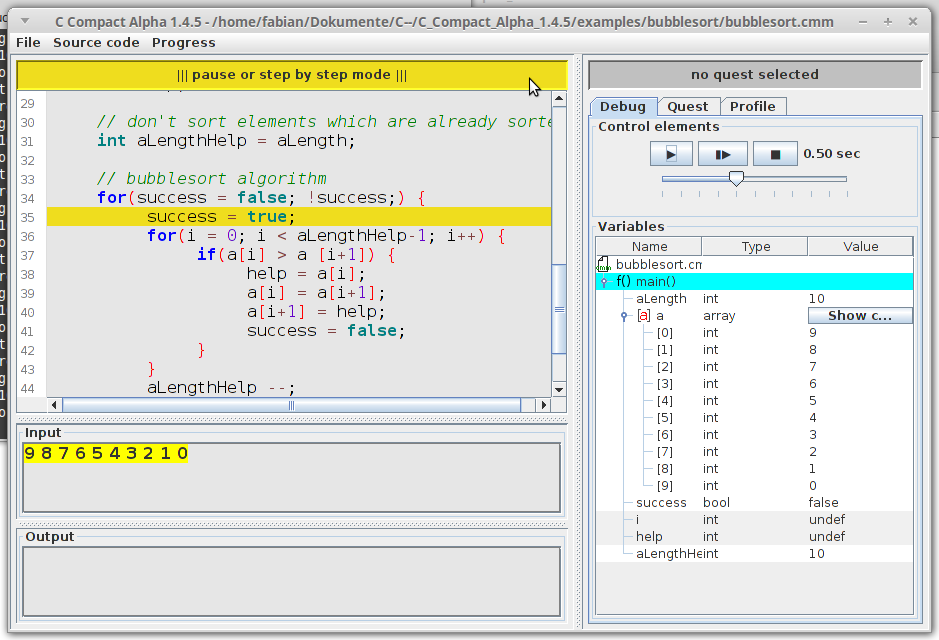
\includegraphics[width=0.7\textwidth]{./media/images/gui/main/CCompactAlpha1-4-5-guimain.png}
  \caption{Aufbau des Hauptfensters}
  \label{fig:gui-main-1}
\end{figure}

\subsection{Implementierung}
\label{sec:gui-main-impl}
Das Hauptfenster selbst ist in der Klasse \textbf{GUImain} implementiert. Diese Klasse implementiert, da sie ein Hauptfenster regelt, das Interface \textbf{GUIExecutable}. Zum Starten der Entwicklungsumgebung muss immer ein Objekt dieser Klasse angelegt werden. Im Konstruktor muss eine Referenz auf ein Einstellungsobjekt der Klasse \textbf{GUImainSettings} übergeben werden. In diesem Objekt werden alle Einstellungen des Benutzers gespeichert.

Wenn C Compact ohne Benutzerprofil gestartet werden soll, wird als Parameter \textbf{null} übergeben. In diesem Fall können keine Quests gestartet werden, alle anderen Funktionen wie etwa der Debugger sind aber verfügbar.
%TODO ref GUImainSettings

\begin{lstlisting}[language=JAVA]
	/**
	 * Constructor requires specific configuration for the window (settings)
	 * 
	 * @param settings Configuration object for the main GUI.
	 */
	public GUImain(GUImainSettings settings) {
		this.settings = settings;
	}
\end{lstlisting}

Um das Hauptfenster zu initialisieren und C Compact zu starten, muss danach die Methode \textbf{void start(boolean test)} aufgerufen werden. Diese Methode wurde vom Interface GUIExecutable übernommen. Als Parameter sollte normalerweise \textbf{false} übergeben werden. Wenn \textbf{true} übergeben wird, wird das Fenster gleich nach dem Initialisieren geschlossen. Diese Funktion wird für automatisierte Tests mit ANT verwendet.
%TODO ref ant tests

\begin{lstlisting}[language=JAVA]
	/**
	 * Initializes and launches the main GUI and therefore the main part of the
	 * program. <b>This is not the static main function!</b> Running this method
	 * requires calling a constructor with configuration data before (see above
	 * in code).
	 * 
	 * @param test
	 *            TRUE if program shall exit after init (for GUI test)
	 */
	@Override
	public void start(boolean test) {
		.
		.
		.
			
		// Initialize the window
		this.jFrame = new JFrame(VERSION);
		this.jFrame.setDefaultCloseOperation(JFrame.DO_NOTHING_ON_CLOSE);
		this.jFrame.getContentPane().setPreferredSize(new Dimension(800, 500));
		this.jFrame.setMinimumSize(new Dimension(600, 400));
		
		.
		.
		.
		
		// Exit if this was just a test
		if (test)
			System.exit(0);
	}
\end{lstlisting}

Außerdem implementiert die Klasse GUImain die Methode \textbf{saveAndDispose()} des Interfaces \textbf{GUIExecutable}. Diese Methode speichert alle Einstellungen und Daten des Benutzers und beendet das Programm.

\begin{lstlisting}[language=JAVA]
	@Override
	public void saveAndDispose() {
		this.getSaveManager().directSave();
		this.getSettings().writeXMLsettings();
		this.dispose();
	}
\end{lstlisting}

\section{Linker Teil der Benutzeroberfläche}
Zum linken Bereich der Benutzeroberfläche gehören Textfelder für Ein- und Ausgabedaten des CMM-Programmes, das Textfeld für den Source Code, sowie ein farbiges Panel, das den aktuellen Zustand der Benutzeroberfläche visualisiert.

Die größe der Elemente kann angepasst werden, indem die Grenzbalken mit der Maus verschoben werden. In Kapitel \ref{sec:gui-main} wurde das JSplitPane bereits erwähnt. Ein SplitPane enthält immer zwei Elemente\footnote{https://docs.oracle.com/javase/tutorial/uiswing/components/splitpane.html}, die durch den verschiebbaren Balken getrennt werden. In diesem Fall werden zwei verschachtelte SplitPanes verwendet. Das äußere Panel enthält einerseits das Zustandspanel (siehe Kapitel \ref{sec:gui-main-left-zust}) und das Textfeld für den Source Code (siehe Kapitel \ref{sec:gui-main-left-code}), andererseits auch ein zweites SplitPane, das Ein- und Ausgabefeld trennt (Kapitel \ref{sec:gui-main-left-io}).
%TODO add doc for JSplitPane

\subsection{Allgemeine Implementierung}
Der gesamte linke Teil der Benutzeroberfläche ist in der Klasse \textbf{GUIleftPanel} im Packet \textbf{at.jku.ssw.cmm.gui} implementiert. Ein Objekt dieser Klasse wird beim Starten von C Compact von \textbf{GUImain} initialisiert.

Für die Kommunikation mit anderen Klassen wurden einige Methoden implementiert, die wichtigsten werden in Tabelle \ref{tab:gui-main-left-methods}

\def\arraystretch{1.6}
\begin{table}
\begin{tabularx}{\columnwidth}{l|p{9cm}}
\textbf{Name}&\textbf{Beschreibung}\\
\hline
\hline
public JSplitPane init(...)&Initialisiert diesen Teil der Benutzeroberfläche und gibt eine Referenz auf das Hauptelement zurück\\
\hline
public void setReadyMode()&\multirow{4}{*}{\parbox{9cm}{Ändert den Modus des Zustandpanels, Siehe Kapitel \ref{sec:gui-main-left-zust}}}\\
public void setErrorMode(...)&\\
public void setRunMode()&\\
public void setPauseMode()&\\
\hline
public void lockInput()&\multirow{2}{*}{\parbox{9cm}{Sperrt und ermöglicht Eingabe in eines der Textfelder, Siehe Kapitel \ref{sec:gui-main-left-zust}}}\\
public void unlockInput()&\\
\hline
public void setOrientation(...)&Ändert die Anordnung der Elemente in diesem Teil der Benutzeroberfläche, Siehe Kapitel \ref{sec:gui-main-left-ord} und ...\\
\hline
public void updateFontSize()&Ändert die Schriftgröße in allen Textfeldern, Siehe Kapitel ...
\end{tabularx}
\caption{Die wichtigsten Methoden der Klasse \textbf{GUIleftPanel}}\label{tab:gui-main-left-methods}
\end{table}
%TODO ref GUIProperties

Die Textfelder in diesem Teil der Benutzeroberfläche werden mit statischen Methoden initialisiert, die in der Klasse \textbf{InitLeftPanel} im Package \textbf{at.jku.ssw.cmm.gui.init} zu finden sind. Im Folgenden wird bei dem jeweiligen Element erwähnt, in welcher Methode es initialisiert wird.

\subsection{Anordnung der Elemente}
\label{sec:gui-main-left-ord}

Um C Compact für alle Bildschirmformate optimal anzupassen, sind in den Einstellungen unterschiedliche Optionen zur Anordnung der Elemente im linken Panel zu finden. Die Abbildungen \ref{fig:gui-main-left-o1} bis \ref{fig:gui-main-left-o4} zeigen die möglichen Konfigurationen.
%TODO ref GUIProperties

\begin{figure}
\centering
	\begin{minipage}{0.45\textwidth}
		\centering
		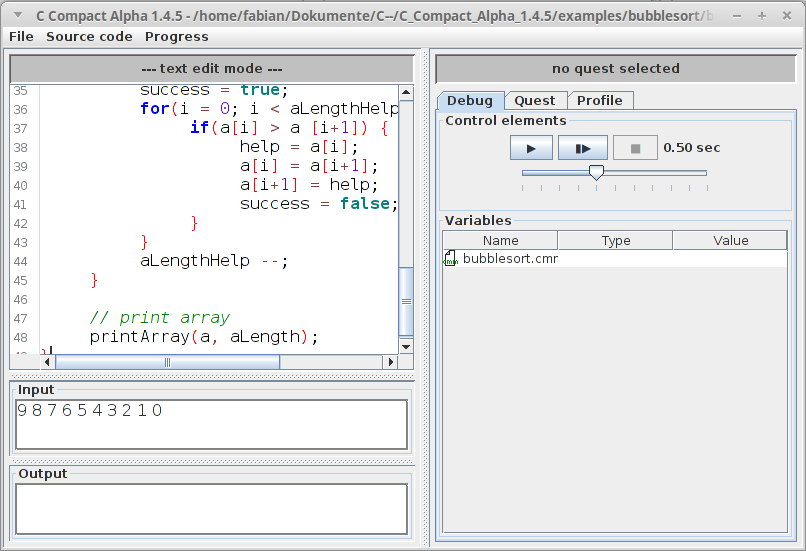
\includegraphics[width=1.0\textwidth]{./media/images/gui/main/orientations/CCompact-gui-1.png}
		\caption{Classic Vertical}\label{fig:gui-main-left-o1}
	\end{minipage}\hfill
	\begin{minipage}{0.45\textwidth}
		\centering
		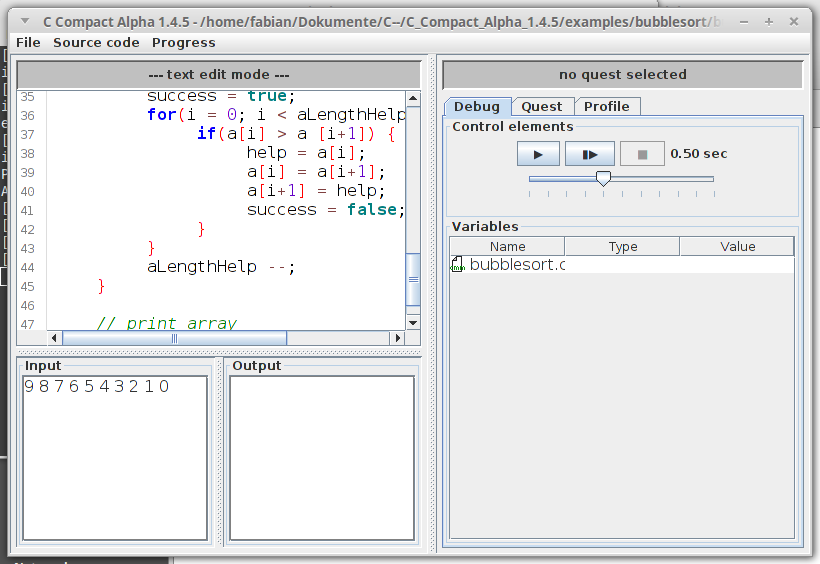
\includegraphics[width=1.0\textwidth]{./media/images/gui/main/orientations/CCompact-gui-2.png}
		\caption{Classic Horizontal}\label{fig:gui-main-left-o2}
	\end{minipage}
\end{figure}

\begin{figure}
\centering
	\begin{minipage}{0.45\textwidth}
		\centering
		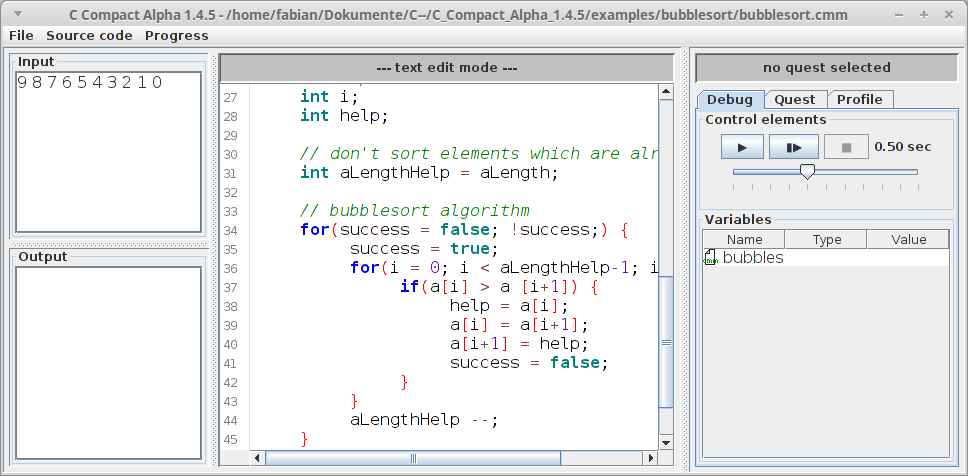
\includegraphics[width=1.0\textwidth]{./media/images/gui/main/orientations/CCompact-gui-3.png}
		\caption{Widescreen Central}\label{fig:gui-main-left-o3}
	\end{minipage}\hfill
	\begin{minipage}{0.45\textwidth}
		\centering
		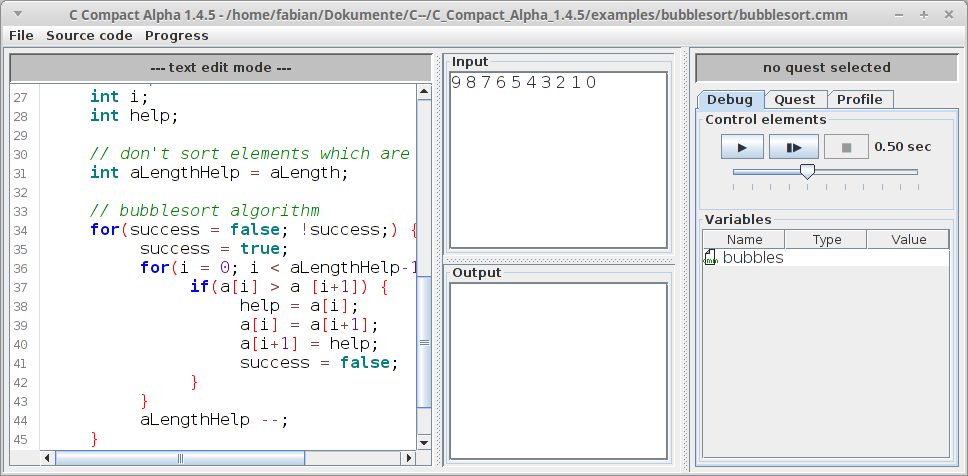
\includegraphics[width=1.0\textwidth]{./media/images/gui/main/orientations/CCompact-gui-4.png}
		\caption{Widescreen Left}\label{fig:gui-main-left-o4}
	\end{minipage}
\end{figure}

Wie zu Beginn dieses Kapitels bereits beschrieben wurde, ist der linke Teil der Benutzeroberfläche mit zwei verschachtelten JSplitPanes organisiert. Für einfache Änderungen am Aufbau der benutzeroberfläche reicht es, die Orientierung eines SplitPanes zu verändern:

\begin{lstlisting}[language=JAVA]
	// Trennbalken ist vertikal
	splitPanel.setOrientation(JSplitPane.VERTICAL_SPLIT);
	
	// Trennbalken ist horizontal
	splitPanel.setOrientation(JSplitPane.HORIZONTAL_SPLIT);
\end{lstlisting}

Mit der Methode \textbf{setOrientation} kann die Anordnung der Elemente im linken Panel verändert werden. Für die dritte mögliche Anordnung (Abbildung \ref{fig:gui-main-left-o3}, ,,Widescreen Central'') müssen die Elemente des äußeren Panels allerdings vertauscht werden. Deshalb wird bei jedem Wechsel auf diese Konfiguration die private Methode ,,swap'' aufgerufen. Wenn als Parameter \textbf{true} übergeben wird, werden die Elemente ausgetauscht, ansonsten werden die Komponenten wieder auf ihre Ausgangsposition geracht.

\begin{lstlisting}[language=JAVA]
	private void swap(boolean def) {
		
		// Reset splitPane
		this.outerPane.setTopComponent(null);
		this.outerPane.setBottomComponent(null);
		
		// Decide what to do
		if( def ) {
			this.outerPane.setTopComponent(this.jSourceCodeContainer);
			this.outerPane.setBottomComponent(this.innerPane);
		}
		else {
			this.outerPane.setBottomComponent(this.jSourceCodeContainer);
			this.outerPane.setTopComponent(this.innerPane);
		}
	}
\end{lstlisting}

\subsection{Zustandspanel}
\label{sec:gui-main-left-zust}
%TODO ref GUI states
%TODO ref right state panel

\begin{figure}[htbp] 
  \centering
     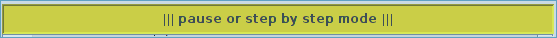
\includegraphics[width=0.7\textwidth]{./media/images/gui/main/CCompact-gui-left-panel.png}
  \caption{Das Zustandspanel während des Debuggens}
  \label{fig:gui-main-left-panel}
\end{figure}

Die Benutzeroberfläche der Entwicklungsumgebung kann vier unterschiedliche Zustände annehmen. Diese Zustände beziehen sich nur auf die Basisfunktionen der Entwicklungsumgebung und des Debuggers, nicht aber auf den Zustand der zu bearbeitenden Quest. Es sind folgende Zustände möglich:
\begin{enumerate}
\item \textbf{Editormodus:} Der Benutzer kann den Source Code wie bei einem Texteditor bearbeiten. Auch Eingabedaten für den Debugger können eingegeben werden. Dies ist der Standardzustand, das Zustandspanel ist grau.
\item \textbf{Fehlermodus:} Es ist ein Fehler im Source Code des Benutzers aufgetreten. Der Fehler wurde entweder im Präprozessor, im Compiler oder im Interpreter erkannt. Das Zustandspanel ist rot und zeigt zusätzliche Informationen zum Fehler, wie etwa die Art des Fehlers und die Zeile, in der der Fehler aufgetreten ist\footnote{Unter Umständen wird nicht die richtige Zeile erkannt, sondern eine darauffolgende Zeile markiert.}. Im rechten Teil des Hauptfensters wird eine detaillierte Beschreibung des Fehlers gezeigt. In diesem Modus kann der Source Code bearbeitet werden, um den Fehler zu beheben.
%TODO ref right panel -> Fehleranzeige
%TODO ref compiler errors -> footnote 

Der Text im Zustandspanel wird im Fehlermodus aus folgenden Informationen zusammengesetzt:
\begin{enumerate}
\item \textbf{Präfix:} Beschreibender Text am Beginn der Nachricht.
\item \textbf{Dateiname:} Wird nur angegeben, wenn der Fehler in einer externen Datei oder einer Bibliothek aufgetreten ist.
\item \textbf{Zeilennummer:} Die Zeile, in der der Fehler aufgetreten ist.
\item \textbf{Postfix:} Beschreibender Textteil am Ende der Nachricht. Dies ist in manchen Sprachen notwendig, um grammatikalisch vollständige Sätze konstruieren zu können (Siehe Beispiel unten).
\end{enumerate}

Die Fehlernachricht wird mit folgendem Code zusammengesetzt. Dieser Teil stammt aus der Funktion \textbf{setErrorMode} in der Klasse \textbf{GUIleftPanel}:

\begin{lstlisting}[language=JAVA]
	// Setting error text for state panel
	this.jStateLabel.setText("<html>! ! ! " +
		// Error title prefix (if available)
		(title[0] == null ? _("error") : title[0]) +
		// File name (if available)
		(file == null || file != "main" ? "" : " in file " + file) + " " +
		// Error line (if available)
		(line >= 0 ? _("in line") + " " + (int)objLine[1] : "") +
		// Error title postfix (if available)
		(title[1] == null ? "" : " " + title[1]) +
	" ! ! !</html>");
\end{lstlisting}

\textbf{Beispiel:}
\[
\underbrace{Semikolon}_{Praefix} \underbrace{in der Datei stdio.h}_{Datei} \underbrace{in Zeile 15}_{Zeilenangabe} \underbrace{(oder vorher) vergessen.}_{Postfix}
\]

Präfix und Postfix können im Head der der Fehlerbeschreibungsdatei definiert werden. Für jeden bekannten Fehler gibt es ein eigenes HTLM-Dokument, das einen entsprechenden Beschreibungstext enthält. Diese Fehlerdateien sind im Ordner \textbf{error} im C Compact Programmordner zu finden.
%TODO ref guirightpanel -> error documents

\begin{lstlisting}[language=HTML]
<head>
	<prefix>Semikolon</prefix>
	<postfix>(oder vorher) vergessen</postfix>
</head>
\end{lstlisting}

\item \textbf{Schritt für Schritt debuggen:} Der Debugger kann grundsätzlich in zwei unterschiedlichen Modi ausgeführt werden. In diesem Fall wird das Programm so ausgeführt, dass der Benutzer jeden Schritt des Interpreters selbst initiieren muss (durch Druck auf den "Nächster Schritt"-Button oder die Taste F6). Hier ist das Zustandspanel gelb gefärbt. Das Bearbeiten des Source Code ist während der Laufzeit nicht möglich.
%TODO ist F6 korrekt???
%TODO refer to debugger

\item \textbf{Austomatisches debuggen:} Die andere Möglichkeit ist, den Interpreter in gewissen Zeitabständen selbst weiterspringen zu lassen. Auch hier ist das Bearbeiten des Source Code nicht möglich. Das Zustandspanel ist grün.
\end{enumerate}

Das Zustandspanel wird in der Methode \textbf{init()} der Klasse \textbf{GUIleftPanel} initialisiert.

\subsection{Textfeld für den Source Code}
\label{sec:gui-main-left-code}
Das Feld für den Source Code wurde als \textbf{RSyntaxTextArea}\footnote{http://bobbylight.github.io/RSyntaxTextArea/} implementiert. Dieses Projekt wurde von Robert Futrell veröffentlicht und steht unter einer modifizierten BSD-Lizenz\footnote{https://github.com/bobbylight/RSyntaxTextArea/blob/master/src/main/dist/RSyntaxTextArea.License.txt}.

Das verwendete Textfeld ermöglicht Syntax Highlighting für viele bekannte Programmiersprachen. Anfangs haben wir den Standardhihglighter für C-Code verwendet; seit der Version Alpha 1.2 wird ein eigens angepasster Syntax Highlighter verwendet. Dadurch werden auch Funktionen und Schlüsselwörter, die nur in C Compact vorkommen, richtig markiert.
%TODO ref Versionsgeschichte
%TODO ref JFlex/Syntax Highlighter [pointhi]
%TODO ref settings -> font size

RSyntaxTextArea stellt noch eine Reihe weiterer praktischer Funktionen zur Verfügung, wie etwa das einklappen (verstecken) von Kommentaren oder Funktionsrümpfen. Manche Features, wie etwa automatische Vervollständigung beim Tippen oder das Erkennen von gleichen Variablennamen haben wir vorerst deaktiviert, um Probleme zu vermeiden und die Benutzeroberfläche nicht zu überfüllen.
%TODO Letzten Satz nochmal lesen

\begin{figure}[htbp] 
  \centering
     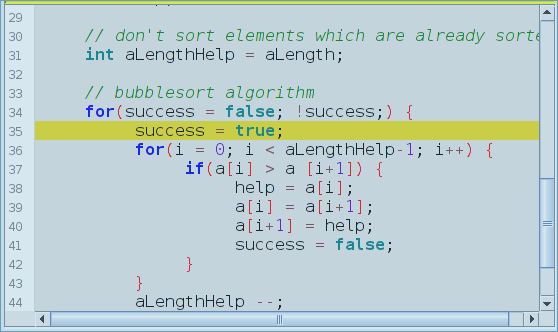
\includegraphics[width=0.7\textwidth]{./media/images/gui/main/CCompact-gui-left-code.png}
  \caption{Das Textfeld für den Source Code}
  \label{fig:gui-main-left-code}
\end{figure}

Die Zeile, in der sich der Cursor befindet, wird durch einen Farbigen Balken markiert. Dieser Balken hat, je nach Modus des Debuggers, die selbe Farbe wie das Zustandspanel (siehe Kapitel \ref{sec:gui-main-left-zust}).

Dieses Textfeld wird mit der statischen Methode \textbf{initCodePane()} der Klasse \textbf{InitLeftPanel} initialisiert. Die Methode wird beim Erstellen des linken Teils der Benutzeroberfläche aufgerufen.

\subsection{Ein- und Ausgabetextfeld}
\label{sec:gui-main-left-io}
%TODO add picture of text pane while reading input data
%TODO ref settings -> font size

In diesem Textfeld werden Daten eingegeben, die vom Interpreter während der Laufeit eingelesen werden. Jedes Zeichen kann nur einmal eingelesen werden; bereits eingelesene Zeichen werden gelb hinterlegt. Die Ausgabedaten werden in einem separaten Textfeld dargestellt.

In C Compact gibt es für Ein- und Ausgabe keine Konsole, wie sie bei einfachen programmen meist verwendet wird. Bei unseren Versuchen hat sich gezeigt, dass dies die Schülerinnen und Schüler kaum stört. Besonders beim Entwicklen eines Algorithmus ist diese Methode der Ein- und Ausgabe besonders hilfreich, da die Eingabedaten nicht immer wieder eingegeben werden müssen.
%TODO ref Versuche

Dem Intrepreter muss immer ein Objekt, welches das Interface \textbf{StdInOut} aus dem Packet \textbf{at.jku.ssw.cmm.debugger} implementiert, übergeben werden. In diesem Interface befinden sich Methoden zur Ein- und Ausgabe. Diese Methoden werden vom Interpreter aufgerufen, wenn im Programm Anweisungen zur Ein- oder Ausgabe vorkommen.
%TODO ref interpreter, debugging listener, ...

\begin{lstlisting}[language=JAVA]
public interface StdInOut {
	public char in() throws RunTimeException;
	public void out(char arg0);
}
\end{lstlisting}

%TODO ref ????
Für den Debugger wurde die Ein- und Ausgabe in der Klasse \textbf{IOstream} im Packet \textbf{at.jku.ssw.cmm.debugger} implementiert. Die (gekürzte) Programmierung sieht wie folgt aus:

\begin{lstlisting}[language=JAVA]
@Override
public char in() throws RunTimeException {

	char c;
	try {
		// Read and remove next character
		c = this.inputStream.get(0);
		this.inputStream.remove(0);
	} catch (Exception e) {
		// Throw interpreter runtime error if no more input data available
		throw new RunTimeException("no input data", null, 0);
	}
	
	//Highlight the character read
	this.main.getLeftPanel().increaseInputHighlighter();
	
	return c;
}

@Override
public void out(final char arg0) {

	java.awt.EventQueue.invokeLater(new Runnable() {
		public void run() {
			// Add given character to output text area of the main GUI
			main.getLeftPanel().outputStream("" + arg0);
		}
	});
}
\end{lstlisting}

Da der Interpreter in einem separaten Thread ausgeführt wird, muss die Ausgabe der übergebenen Daten in den \textbf{Event Dispatcher Thread} eingereiht werden. Für die Eingabedaten inst das nicht notwendig, da der Eingabestring in einer lokalen Variable dieses Objektes gespeichert ist, auf den kein anderer Thread zugreifen kann.
%TODO ref EDT, thread problem

Um das Markieren der bereits eingelesenen Daten und das Aussehen des Eingabedatenfeldes richtig zu organisieren, wurde das Element \textbf{JInputDataPane} erstellt. Diese Klasse erbt von dem zuvor verwendeten \textbf{JTextPane}\footnote{http://docs.oracle.com/javase/7/docs/api/javax/swing/JTextPane.html}. Die Klasse JInputDataPane ist im Package \textbf{at.jku.ssw.cmm.gui.init} zu finden. 

Die verwendeten Textfelder werden mit den statischen Methoden \textbf{initInputPane()} und \textbf{initOutputPane()} der Klasse \textbf{InitLeftPanel} initialisiert.

\section{Rechter Teil der Benutzeroberfläche}
Der rechte Teil der Benutzeroberfläche besteht aus einem Zustandspanel für die aktuelle Aufgabe (Quest) und einem Panel mit mehreren Registerkarten, die unterschiedliche Bedienelemente enthalten, zum Beispiel für den Debugger.

Ähnlich wie der linke Teil der Benutzeroberfläche besitzt auch dieser Bereich eine eigene Klasse. Die Klasse \textbf{GUIrightPanel} im Paket \textbf{at.jku.ssw.cmm.gui} bildet eine Schnittstelle zwischen dem Hauptteil der Benutzeroberfläche (der Klasse \textbf{GUImain}, siehe Kapitel \ref{gui-main}) und den Komponenten, die in den Registerkarten des rechten Panels eingebettet sind.
%TODO letzten Satz nochmal lesen

Wie bei der Klasse \textbf{GUIleftPanel} wird die Benutzeroberfläche selbst mit der Methode \textbf{init} augerufen. Als Parameter wird eine Referenz auf \textbf{GUImain} übergeben, der Rückgabewert ist das fertig initialisierte rechte Panel.

In den Registerkarten können folgende Inhalte vorhanden sein:
\def\arraystretch{1.6}
\begin{table}
\begin{tabularx}{\columnwidth}{l|p{3cm}|p{6cm}|l}
\textbf{Name}&\textbf{Sichtbar}&\textbf{Beschreibung}&\textbf{Siehe Kapitel}\\
\hline
Debug&Immer&Enthält Elemente zum Bedienen des Debuggers&0.0.0\\%TODO ref Debugger GUI
Error&Fehler aufgetreten&Zeigt detaillierte Informationen zu einem beim Debuggen an&0.0.0\\%TODO ref compiler, interpreter errors
Quest&Questsystem aktiv&Zeigt die aktuelle Aufgabenstellung an und ermöglicht das Überprüfen der Aufgabe&0.0.0\\%TODO ref Questsystem
Profile&Questsystem aktiv&Zeigt das Profil des Benutzers: Benutzerbild, Name und Auszeichnungen&0.0.0%TODO ref Profile, profilePanel
\end{tabularx}
\caption{Registerkarten im rechten Teil des Hauptfensters}\label{tab:gui-main-right-reg}
\end{table}
%TODO add chapter references in last column

Da die Inhalte dieser Panele in den Bericht spezifischer Funktionen von C Compact fallen, werden Aufbau, Implementierung und Funktion dieser Komponenten in anderen Teilen dieser Dokumentation beschrieben.

\subsection{Zustandspanel des Questsystems}
Wie auch das Zustandspanel des Debuggers, das in Kapitel \ref{sec:gui-main-left-zust} beschrieben wurde, visualisiert dieses Panel einen Zustand. Allerdings bezieht sich diese Oberfläche nur auf das Questsystem und ist daher auch nur gemeinsam mit diesem Verfügbar (In Kapitel \ref{sec:gui-main-impl} wurde dargelegt, wie C Compact ohne den Funktionen des Questsystems gestartet werden kann). Es ist wichtig zu erwähnen, dass die Zustände des Questsystems vollkommen unabhängig von denen des Debuggers sind.
%TODO ref quest system, quest tester

Folgende Zustände können angezeigt werden:
\begin{enumerate}
\item \textbf{Keine Quest ausgewählt (Idle):} Zu Beginn hat der Benutzer noch keine Aufgabe ausgewählt, das Zustandspanel ist grau.
\item \textbf{Quest wird bearbeitet:} Während der Benutzer eine ausgewählte Aufgabe bearbeitet, ist das Panel blau.
\item \textbf{Quest wird getestet:} Wenn der Benutzer überprüfen will, ob er eine Aufgabe richtig erfüllt hat startet er einen Test. Während des Tests wird das Zustandspanel gelb, im Regelfall ist dieser Status aber sehr kurz. Wenn während des Tests ein Fehler auftritt (wie etwa eine Endlosschleife), kann der Test in diesem Zustand abgebrochen werden.
%TODO ref Quest test, quest test panel
\item \textbf{Test erfolgreich:} Verläuft der Test erfolgreich, wird das Zustandspanel grün.
\item \textbf{Test fehlgeschlagen:} In diesem Fall ist entweder ein Fehler im Source Code des Benutzers erkannt worden (eine Detaillierte Beschreibung wird im Fehlerpanel angezeigt, siehe Kapitel \ref{}) oder das Programm des Benutzers erfüllt die gestellte Aufgabe nicht. Der Benutzer hat die Möglichkeit, seinen Code zu überarbeiten.
%TODO finish ref
\end{enumerate}

Der angezeigte Zustand wird mit folgenden Methoden der Klasse \textbf{GUIrightPanel} initialisiert. Diese Methoden sind wirkungslos, wenn das Questsystem deaktiviert ist.
\begin{lstlisting}[language=JAVA]
public void setIdleMode();
public void setQuestMode(String title); // Name der Quest wird übergeben
public void setTestMode();
public void setSuccessMode();
public void setFailedMode();
\end{lstlisting}

%TODO add refs to the following four subsections
\subsection{Registerkarte ,,Debug''}
Diese Registerkarte ist immer an der ersten Stelle und jederzeit verfügbar. Im oberen Teil befindet sich ein Panel mit Bedienelementen des Debuggers, darunter werden die Variablen im Programm des Benutzers während der Laufzeit des Interpreters dargestellt.

Eine Referenz auf das Panel in dieser Registerkarte wird von folgender Methode übergeben:
\begin{lstlisting}[language=JAVA]
public GUIdebugPanel getDebugPanel() {
	return this.debugPanel;
}
\end{lstlisting}

\subsection{Registerkarte ,,Error''}
Wenn beim Debuggen ein Fehler im Compiler, Präprozessor oder Interpreter auftritt, wird dieses Panel sichtbar. Außerdem werden Fehler angezeigt, die beim Überprüfen einer Quest auftreten, sofern der Fehler durch den Source Code des Benutzers aufgetreten ist. Ist der Fehler behoben und wurde das Programm erfolgreich ausgeführt, verschwindet diese Registerkarte automatisch.

Mit folgender Methode werden Fehlernachrichten eingeblendet. Als Parameter wird die Fehlernachricht des Compiler, Präprozessor oder Interpreter übergeben, der Rückgabewert ist der Name (Präfix und Postfix) des Fehlers, wie er im Zustandspanel des Debuggers angezeigt wird. Siehe dazu Kapitel \ref{sec:gui-main-left-zust}.
\begin{lstlisting}[language=JAVA]
public String[] showErrorPanel(String errorCode);
\end{lstlisting}

Eine Detaillierte Beschreibung dieser Methode und der Verwaltung von Fehlerdokumenten ist in Kapitel \ref{} zu finden.

\subsection{Registerkarte ,,Quest''}
In dieser Registerkarte werden Informationen und Bedienelemente zum Ausführen einer Aufgabe des Questsystems (siehe Kapitel \ref{}) angezeigt.

Eine Referenz auf das Panel in dieser Registerkarte wird von folgender Methode übergeben:
\begin{lstlisting}[language=JAVA]
public GUITestPanel getTestPanel(){
	return this.testPanel;
}
\end{lstlisting}

%TODO also mention this in chapter "quest panel"
Anmerkung: Dieses Panel wird - vor Allem im Source Code von C Compact - auch als ,,testPanel'' bezeichnet, da der Benutzer mit Elementen dieses Komponenten überprüfen kann, ob er die aktuelle Aufgabe richtig gelöst hat.

\subsection{Registerkarte ,,Profile''}
Hier werden Informationen zum aktuellen Spielerprofil angezeigt. Siehe Kapitel \ref{}.

Eine Referenz auf das Panel in dieser Registerkarte wird von folgender Methode übergeben:
\begin{lstlisting}[language=JAVA]
public ProfilePanel2 getProfilePanel() {
	return this.questPanel;
}
\end{lstlisting}

\section{Menüleiste}
\label{sec:gui-main-menu}
Menüs sind bei der Gestaltung einer Benutzeroberfläche nahezu unerlässlich. Eine Menüleiste, bzw. ein Menü erleichtert dem Benutzer die Orientierung, da alle Funktionen auf einen Blick zu finden sind. Die Menüleiste wird auch in den \emph{Common User Access}\footnote{http://de.wikipedia.org/wiki/Common\_User\_Access} Richtlinien für die Gestatlung von Benutzeroberflächen definiert; diese Standards wurden 1989 von der Firma IBM festgelegt. Diese Standards sind mittlerweile weit verbreitet und wurden in einer Reihe von Systemen umgesetzt.

Die Menüleiste wird in der statischen Methode \textbf{initFileM()} in der Klasse \textbf{at.jku.ssw.cmm.gui.init.InitMenuBar} angelegt. Die Tastaturkürzel - \emph{,,Keyboard Shortcuts''} - zum Beispiel \emph{Strg + S} zum Speichern, werden ebenfalls hier definiert. Beim Verwenden eines Tastaturkürzels wird der Event Listener des zugehörigen Menüeintrages aufgerufen.
%TODO ref to keyboard shortcuts in GUIcontrolPanel

Initialisieren eines Menüeintrages:
\begin{lstlisting}[language=JAVA]
// Menüeintrag wird initialisiert
JMenuItem openMI = new JMenuItem(_("Open"));

// Menüeintrag wird zum Menü hinzugefügt
fileM.add(openMI);

// Mit dem Action Listener verknüpfen, sodass dieser beim Anklicken des Menüs aufgerufen wird
openMI.addActionListener(listener.openHandler);

// Mit dem Keyboard Shortcut verknüpfen
openMI.setAccelerator(KeyStroke.getKeyStroke(KeyEvent.VK_O, ActionEvent.CTRL_MASK));

// Eintrag zur MenuBarControl hinzufügen
menuBarControl.add(newMI);
\end{lstlisting}

Die Events der Menüleiste werden in der Klasse \textbf{at.jku.ssw.cmm.gui.event.MenuBarEventListener} abgewickelt. Diese Klasse enthält Methoden, die bestimmte Aktionen abwickeln und innere Klassen, die einen Event Listener implementieren und diese Methoden aufrufen. Diese Aufteilung ist nötig, da bestimmte Aktionen auch von anderen instanzen aufgerufen werden können (zum Beispiel wird auch gespeichert, wenn der Benutzer C Compact schließt).

\subsection{Aktivieren und Deaktivieren von Menüeinträgen}
\label{sec:gui-main-menu-ctrl}
Da während der Debugger ausgeführt wird keine Aktionen erlaubt sind, die den Text im Source Code Textfeld ändern (Siehe Kapitel \ref{sec:gui-main-left-code}), werden bestimmte Menüeinträge aktiviert oder deaktiviert, wenn sich der Status des Debuggers ändert (Siehe Kapitel \ref{sec:gui-main-left-zust}). Diese Aktionen werden in der Klasse \textbf{at.jku.ssw.cmm.gui.MenuBarControl} zusammengefasst. Diese Klasse enthält eine Liste, in der alle Menüeinträge referenziert werden, die beim Ausführen des Debuggers deaktiviert werden sollen. Mit der Methode \textbf{add()} werden Objekte in diese Liste eingetragen.
\begin{lstlisting}[language=JAVA]
public void add(JMenuItem mi){
	this.list.add(mi);
}
\end{lstlisting}

Mit den Methoden \textbf{lockAll()} und \textbf{unlockAll()} werden diese Menüeinträge dann deaktiviert oder aktiviert.

\begin{lstlisting}[language=JAVA]
public void lockAll();
public void unlockAll();
\end{lstlisting}

Des Weiteren kann in dieser Kontrollklasse ein Menüeintrag definiert werden, der eine Liste der zuletzt geöffneten Dateien enthält. Mit der Methode \textbf{setRecentMenu} wird dieser Menüeintrag definiert:
\begin{lstlisting}[language=JAVA]
public void setRecentMenu( JMenu mi ){
	this.recentMI = mi;
}
\end{lstlisting}

Dieses Untermenü wird mit der Methode \textbf{updateRecentFiles} aktualisiert. Siehe dazu auch Kapitel \ref{}.
%TODO ref GUImainSettings
\begin{lstlisting}[language=JAVA]
public void updateRecentFiles( List<String> recentFiles, String currentFile );
\end{lstlisting}

Im Untermenü ,,Source Code'' (Siehe Kapitel \ref{}) gibt es Funktionen zum Aufheben bzw. Wiederholen der letzten Aktion (\emph{undo and redo}). Diese Menüeinträge sollen aber nur aktiviert sein, wenn eine solche Aktion tatsächlich möglich ist. Beispielsweise kann nach dem Start des Programmes nichts rückgängig gemacht werden, da noch keine Aktionen durchgeführt wurden. Außerdem dürfen diese Aktionen nicht ausgeführt werden, wenn der Debugger gerade läuft, da der Source Code sonst während der Laufzeit verändert werden würde.

Referenzen auf die beiden entsprechenden Menüeinträge werden in der Klasse MenuBarControl separat gespeichert.
\begin{lstlisting}[language=JAVA]
public void setUndo(JMenuItem undo){
	this.undo = undo;
}

public void setRedo(JMenuItem redo){
	this.redo = redo;
}
\end{lstlisting}

Mit der Methode \textbf{updateUndoRedo()} werden die Zustände dieser Menüeinträge aktualisiert. Als Parameter werden eine Referenz auf das Textfeld mit dem Source Code und eine boolean-Variable übergeben. Letztere ist \textbf{true} wenn der Debugger gerade läuft.
\begin{lstlisting}[language=JAVA]
public void updateUndoRedo( RSyntaxTextArea tArea, boolean running ){
	this.undo.setEnabled(!running & tArea.canUndo());
	this.redo.setEnabled(!running & tArea.canRedo());
}
\end{lstlisting}

\subsection{Menü ,,Datei''}
\label{sec:gui-main-menu-file}
Das wohl gewohnteste Menü in jedem Programm ist das Menü ,,Datei'' In C Compact enthält es neben den grundlegenden Funktionen zum Öffnen oder Speichern einer vorhandenen oder neuen Datei auch noch weitere Funktionen. Der Eintrag ,,Drucken'' verwendet eine Methode, die in der RSyntaxTextArea implementiert ist (Siehe Kapitel \ref{sec:gui-main-left-code}; allerdings treetn bei der Formatiering oft Fehler auf. Wesentlich wichtiger sind die Menüpunkte ,,Einstellungen'' (Siehe Kapitel \ref{}), ,,Sprache'' (Siehe Kapitel \ref{}) und ,,Über C Compact'' (Siehe Kapitel \ref{}). Schließlich gibt es noch dem Menüpunkt ,,Beenden'', C Compact kann aber auch mit der Tastenkombination \emph{Alt + F4} (diese Kombination ist in den meisten Betriebssystemen und Oberflächen bereits standardmäßig integriert) oder über entsprechende Bedienelemente im Fensterrahmen geschlossen werden.
%TODO ref sprache, einstellungen, about

\subsection{Menü ,,Source Code''}
Dieses Menü würde in den meisten Programmen dem Menü ,,Bearbeiten'' entsprechen. Allerdings beziehen sich die Menüeinträge wie ,,Kopieren'', ,,Einfügen'', ,,Rückgängig'', etc. immer auf das Textfeld für den Source Code - wir wollen mit dem Menünamen also Verwechslungen vermeiden - und andererseits enthält dieses Menü auch Einträge zum Steuern des Debuggers. Diese Einträge werden vom Benutzer kognitiv mit dem Source Code verknüpft.

\subsection{Menü ,,Fortschritt''}
Dieses Menü enthält Einträge, die das Questsystem (Siehe Kapitel \ref{}) betreffen. Mit ,,Profil Wählen'' Wird C Compact beendet und der Launcher (Siehe Kapitel \ref{}) gestartet, sodass der Benutzer ein anderes Profil wählen kann. Mit dem Befehl ,,Profil Exportortieren'' kann der Benutzer sein Profil an einem anderen Ort speichern (Siehe Kapitel \ref{}). Der Menüeintrag ,,Quest wählen'' öffnet ein Fenster zum Auswählen eines Questpaketes; im Anschluss kann der Benutzer eine Aufgabe zum Bearbeiten wählen (Siehe Kapitel \ref{}). Mit ,,Questpaket importieren'' kann ein Package importiert werden (Siehe Kapitel \ref{} und \ref{}).
%TODO ref Questsystem
%TODO ref launcher
%TODO ref profil exportieren
%TODO ref select quest window
%TODO ref package, import package

